\subsection{Contained class set field values}
\label{subsec:library_of_transformations:instance_level_transformations:contained_class_set_field_values}

\begin{figure}
    \centering
    \begin{subfigure}{0.95\textwidth}
        \centering
        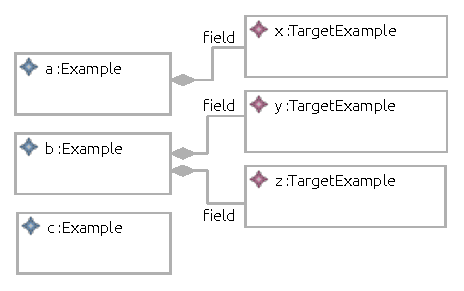
\includegraphics{images/05_library_of_transformations/03_instance_level_transformations/10_contained_class_set_field_values/contained_class_set_field_value.pdf}
        \caption{$Im_{ContainedClassSetField}$ with examples of different nodes with different values for $\type{field}$}
        \label{fig:library_of_transformations:instance_level_transformations:contained_class_set_field_values:visualisation:ecore}
    \end{subfigure}
    \\
    \begin{subfigure}{0.95\textwidth}
        \centering
        % To use this figure in your LaTeX document
% import the package groove/resources/groove2tikz.sty
%
\begin{tikzpicture}[scale=\tikzscale,name prefix=start-]
\node[basic_node] (n0) at (1.805, -0.645) {\ml{\uline{\textit{a}} : \textbf{Example}}};
\node[basic_node] (n1) at (1.805, -1.035) {\ml{\uline{\textit{b}} : \textbf{Example}}};
\node[basic_node] (n2) at (3.750, -0.440) {\ml{\uline{\textit{x}} : \textbf{TargetExample}}};
\node[basic_node] (n3) at (3.745, -0.815) {\ml{\uline{\textit{y}} : \textbf{TargetExample}}};
\node[basic_node] (n4) at (3.740, -1.205) {\ml{\uline{\textit{z}} : \textbf{TargetExample}}};
\node[basic_node] (n5) at (1.800, -1.410) {\ml{\uline{\textit{c}} : \textbf{Example}}};

\path[basic_edge] (n0)  -- node[lab] {\ml{field}} (n2) ;
\path[basic_edge] (n1)  -- node[lab] {\ml{field}} (n4) ;
\path[basic_edge] (n1)  -- node[lab] {\ml{field}} (n3) ;
\end{tikzpicture}

        \caption{$IG_{ContainedClassSetField}$ with examples of different nodes with different values for $\type{field}$}
        \label{fig:library_of_transformations:instance_level_transformations:contained_class_set_field_values:visualisation:groove}
    \end{subfigure}
    \caption{Visualisation of the transformation of field values from containment fields typed by a set of a proper class type}
    \label{fig:library_of_transformations:instance_level_transformations:contained_class_set_field_values:visualisation}
\end{figure}

This section introduces the instance level transformation belonging to the transformation of a containment field of a set of a proper class type. The type level transformation belonging to these fields can be found in \cref{subsec:library_of_transformations:type_level_transformations:contained_class_set_fields}. On the instance level, values for these fields are introduced.

\begin{defin}[Instance model $Im_{ContainedClassSetField}$]
\label{defin:library_of_transformations:instance_level_transformations:contained_class_set_field_values:imod_contained_class_set_field}
Let $Im_{ContainedClassSetField}$ be an instance model typed by $Tm_{ContainedClassSetField}$ (\cref{defin:library_of_transformations:type_level_transformations:contained_class_set_fields:tmod_contained_class_set_field}). Define a set $objects$, which represent the objects that will get a value for the field introduced by $Tm_{DataField}$. Furthermore, define a function $obids$ which maps each of these objects to their corresponding identifier and a function $values$, which maps each of these objects to its value for the field introduced by $Tm_{DataField}$. Please note that $values$ returns a set of objects, as the field allows for this. $Im_{DataField}$ is defined as:
\begin{align*}
Object =\ &objects \cup \bigg(\bigcup_{ob \in objects} values(ob)\bigg)\\
\mathrm{ObjectClass} =\ & \begin{cases}
    (ob, classtype) & \mathrm{if }\ ob \in objects\\
    (ob, containedtype) & \mathrm{if }\ ob \in \bigcup_{ob \in objects} values(ob)
\end{cases}\\
\mathrm{ObjectId} =\ & \begin{cases}
    (ob, obids(ob)) & \mathrm{if }\ ob \in objects
\end{cases}\\
\mathrm{FieldValue} =\ & \begin{cases}
    \Big((ob, (classtype, name)), \big[\type{setof}, \langle [\type{obj}, ob] \mid ob \in values(ob) \rangle\big]\Big) & \mathrm{if }\ ob \in objects
\end{cases} \\
\mathrm{DefaultValue} =\ & \{\}
\end{align*}
\isabellelref{imod_contained_class_set_field}{Ecore-GROOVE-Mapping-Library.ContainedClassSetFieldValue}
\end{defin}

\begin{thm}[Correctness of $Im_{ContainedClassSetField}$]
\label{defin:library_of_transformations:instance_level_transformations:contained_class_set_field_values:imod_contained_class_set_field_correct}
$Im_{ContainedClassSetField}$ (\cref{defin:library_of_transformations:instance_level_transformations:contained_class_set_field_values:imod_contained_class_set_field}) is a valid instance model in the sense of \cref{defin:formalisations:ecore_formalisation:instance_models:model_validity}.
\isabellelref{imod_contained_class_set_field_correct}{Ecore-GROOVE-Mapping-Library.ContainedClassSetFieldValue}
\end{thm}

A visual representation of $Im_{ContainedClassSetField}$ with $objects = \{ob_a, ob_b, ob_c\}$ can be seen in \cref{fig:library_of_transformations:instance_level_transformations:contained_class_set_field_values:visualisation:ecore}. This example is typed by $Tm_{ContainedClassSetField}$ in \cref{fig:library_of_transformations:type_level_transformations:contained_class_set_fields:visualisation:ecore}. In this visualisation, the field value for $ob_a$ is defined as $values(ob_a) = \{ob_x\}$. Furthermore, the value for $ob_b$ is $values(ob_a) = \{ob_y, ob_z\}$. Finally, the value for $ob_c$ is $values(ob_c) = \{\}$, which is allowed because the lower bound of the multiplicity is set 0 by the example. Like the previous transformations for field values, the value needs to be set for all objects that are typed by the class type corresponding to the field. Failing to do so would result in an invalid instance model after it is combined with another model, as the next definition will show. The correctness proof of $Im_{ContainedClassSetField}$ only is already quite involved, but not be included here for conciseness. It can be found as part of the validated Isabelle proofs.

In order to make composing transformation functions possible, $Im_{ContainedClassSetField}$ should be compatible with the instance model it is combined with.

\begin{thm}[Correctness of $\mathrm{combine}(Im, Im_{ContainedClassSetField})$]
\label{defin:library_of_transformations:instance_level_transformations:contained_class_set_field_values:imod_contained_class_set_field_combine_correct}
Assume an instance model $Im$ that is valid in the sense of \cref{defin:formalisations:ecore_formalisation:instance_models:model_validity}. Then $Im$ is compatible with $Im_{ContainedClassSetField}$ (in the sense of \cref{defin:transformation_framework:instance_models_and_instance_graphs:combining_instance_models:compatibility}) if:
\begin{itemize}
    \item All requirements of \cref{defin:library_of_transformations:type_level_transformations:contained_class_set_fields:tmod_contained_class_set_field_combine_correct} are met, to ensure the combination of the corresponding type models is valid;
    \item The class type on which the field is defined by $Tm_{ContainedClassSetField}$ may not be extended by another class type in the type model corresponding to $Im$;
    \item The contained type and the class type cannot be the same, e.g. $classtype \neq containedtype$.
    \item All of the objects in the set $objects$ must already be objects in $Im$;
    \item All of the referenced objects cannot be objects in $Im$, they are newly introduced by $Im_{ContainedClassSetField}$;
    \item All objects typed by the class type on which the field is defined must occur in the set $objects$ and thus have a value in $Im_{ContainedClassSetField}$;
    \item For all of the objects in the set $objects$, the identifier set by $obids$ must be the same identifier as set by $Im$ for that object;
    \item The object ids for the newly introduced objects must be unique with respect to each other and all other objects within $Im$;
    \item For all objects in set $valobjects$, the value set by the $values$ function must be valid and the amount of elements in each value must be within the multiplicity $mul$.
\end{itemize}
\isabellelref{imod_contained_class_set_field_combine_correct}{Ecore-GROOVE-Mapping-Library.ContainedClassSetFieldValue}
\end{thm}

\begin{proof}
Use \cref{defin:transformation_framework:instance_models_and_instance_graphs:combining_instance_models:imod_combine_merge_correct}. It is possible to show that all assumptions hold. Now we have shown that $\mathrm{combine}(Im, Im_{ContainedClassSetField})$ is consistent in the sense of \cref{defin:formalisations:ecore_formalisation:instance_models:model_validity}.
\end{proof}

Please note that all objects referenced by any objects via this field are newly created. They may not exist on the existing model. This is enforced to ensure that the containment relations of objects remain acyclic, which is needed to keep the instance model valid. The proof is not included here for conciseness, but can be found as part of the validated proofs in Isabelle.

The definitions and theorems for introducing values for fields of data types within Ecore are now complete. 

\subsubsection{Encoding as edges and nodes}

In the type level transformation of contained class set fields, a single containment edge type was introduced to encode the values for the containment field. On the instance level, the values for each object will be encoded using this edge type. The encoding corresponding to $Im_{ContainedClassSetField}$ can then be represented as $IG_{ContainedClassSetField}$, defined in the following definition:

\begin{defin}[Instance graph $IG_{ContainedClassSetField}$]
\label{defin:library_of_transformations:instance_level_transformations:contained_class_set_field_values:ig_contained_class_set_field_as_edge_type}
Let $IG_{ContainedClassSetField}$ be the instance graph typed by type graph $TG_{ContainedClassSetField}$ (\cref{defin:library_of_transformations:type_level_transformations:contained_class_set_fields:tg_contained_class_set_field_as_edge_type}). Reuse the set $objects$ from $Im_{ContainedClassSetField}$. Moreover, reuse the functions $obids$ and $values$ from $Im_{ContainedClassSetField}$.

The objects in the set $objects$ are converted to nodes in $Im_{ContainedClassSetField}$. For each of these objects, a edge is created for each referenced object within the value of that field. Each of these edges targets an node that encodes an object that was referenced by the value. Finally, the identity of the objects is defined using $obids$. $IG_{ContainedClassSetField}$ is defined as:
\begin{align*}
N =\ & objects \cup \bigg(\bigcup_{ob \in objects} values(ob)\bigg)\\
E =\ & \bigcup_{ob \in objects} \big\{\big(ob, (\mathrm{ns\_\!to\_\!list}(classtype), \langle name \rangle, \mathrm{ns\_\!to\_\!list}(containedtype)), v\big) \mid v \in values(ob) \big\} \\
\mathrm{ident} =\ & \begin{cases}
    (obids(ob), ob) & \mathrm{if }\ ob \in objects \cup \Big(\bigcup_{ob \in objects} values(ob)\Big)
\end{cases}
\end{align*}
with
\begin{align*}
\mathrm{type}_n =\ & \begin{cases}
    (ob, \mathrm{ns\_\!to\_\!list}(classtype)) & \mathrm{if }\ ob \in objects\\
    (v, \mathrm{ns\_\!to\_\!list}(containedtype)) & \mathrm{if }\ v \in \bigcup_{ob \in objects} values(ob)
\end{cases}
\end{align*}
\isabellelref{ig_contained_class_set_field_as_edge_type}{Ecore-GROOVE-Mapping-Library.ContainedClassSetFieldValue}
\end{defin}

\begin{thm}[Correctness of $IG_{ContainedClassSetField}$]
\label{defin:library_of_transformations:instance_level_transformations:contained_class_set_field_values:ig_contained_class_set_field_as_edge_type_correct}
$IG_{ContainedClassSetField}$ (\cref{defin:library_of_transformations:instance_level_transformations:contained_class_set_field_values:ig_contained_class_set_field_as_edge_type}) is a valid instance graph in the sense of \cref{defin:formalisations:groove_formalisation:instance_graphs:instance_graph_validity}.
\isabellelref{ig_contained_class_set_field_as_edge_type_correct}{Ecore-GROOVE-Mapping-Library.ContainedClassSetFieldValue}
\end{thm}

A visual representation of $IG_{ContainedClassSetField}$ with $objects = \{ob_a, ob_b, ob_c\}$ can be seen in \cref{fig:library_of_transformations:instance_level_transformations:contained_class_set_field_values:visualisation:groove}. This example is typed by $TG_{ContainedClassSetField}$ in \cref{fig:library_of_transformations:type_level_transformations:contained_class_set_fields:visualisation:groove}. In this visualisation, the field value for $ob_a$ is defined as $values(ob_a) = \{ob_x\}$. Furthermore, the value for $ob_b$ is $values(ob_a) = \{ob_y, ob_z\}$. Finally, the value for $ob_c$ is $values(ob_c) = \{\}$. Like the previous field encodings, one needs to set the values for the field for all objects of the encoded class type at once. Failing to do so would result in an invalid instance graph after it is combined with another graph, as the next definition will show. The correctness proof of $IG_{ContainedClassSetField}$ only is already quite involved, but not be included here for conciseness. It can be found as part of the validated Isabelle proofs.

In order to make composing transformation functions possible, $IG_{ContainedClassSetField}$ should be compatible with the instance graph it is combined with.

\begin{thm}[Correctness of $\mathrm{combine}(IG, IG_{ContainedClassSetField})$]
\label{defin:library_of_transformations:instance_level_transformations:contained_class_set_field_values:ig_contained_class_set_field_as_edge_type_combine_correct}
Assume an instance graph $IG$ that is valid in the sense of \cref{defin:formalisations:groove_formalisation:instance_graphs:instance_graph_validity}. Then $IG$ is compatible with $IG_{ContainedClassSetField}$ (in the sense of \cref{defin:transformation_framework:instance_models_and_instance_graphs:combining_instance_graphs:compatibility}) if:
\begin{itemize}
    \item All requirements of \cref{defin:library_of_transformations:type_level_transformations:contained_class_set_fields:tg_contained_class_set_field_as_edge_type_combine_correct} are met, to ensure the combination of the corresponding type graphs is valid;
    \item The node type on which the corresponding field is defined is not extended by other node types within the type graph corresponding to $IG$;
    \item The contained type and the class type cannot be the same, e.g. $classtype \neq containedtype$.
    \item All nodes in $objects$ are also nodes in $IG_{ContainedClassSetField}$;
    \item All nodes referenced by the nodes in $objects$ are not already nodes in $IG_{ContainedClassSetField}$, e.g. the nodes referenced by values are newly introduced;
    \item All nodes typed by the node type on which the field is defined must occur in the set $objects$ and thus have a value in $IG_{ContainedClassSetField}$;
    \item The object ids for the newly introduced objects must be unique with respect to each other and all other objects within $IG$;
    \item For all nodes shared between $IG$ and $IG_{ContainedClassSetField}$, each node must have the same identifier in both $IG$ and $IG_{ContainedClassSetField}$;
    \item For all nodes in set $objects$, the value set by the $values$ function must be valid and the amount of elements in each value must be within the multiplicity $mul$.
\end{itemize}
\isabellelref{ig_contained_class_set_field_as_edge_type_combine_correct}{Ecore-GROOVE-Mapping-Library.ContainedClassSetFieldValue}
\end{thm}

\begin{proof}
Use \cref{defin:transformation_framework:instance_models_and_instance_graphs:combining_instance_graphs:ig_combine_merge_correct}. It is possible to show that all assumptions hold. Now we have shown that $\mathrm{combine}(IG, IG_{ContainedClassSetField})$ is valid in the sense of \cref{defin:formalisations:groove_formalisation:instance_graphs:instance_graph_validity}.
\end{proof}

The next definitions define the transformation function from $Im_{ContainedClassSetField}$ to \\$IG_{ContainedClassSetField}$:

\begin{defin}[Transformation function $f_{ContainedClassSetField}$]
\label{defin:library_of_transformations:instance_level_transformations:contained_class_set_field_values:imod_contained_class_set_field_to_ig_contained_class_set_field_as_edge_type}
The transformation function $f_{ContainedClassSetField}(Im)$ is defined as:
\begin{align*}
N =\ & Object_{Im}\\
E =\ & \bigcup_{ob \in Object_{Im} \land ob \in objects} \big\{\big(ob, (\mathrm{ns\_\!to\_\!list}(classtype), \langle name \rangle, \mathrm{ns\_\!to\_\!list}(containedtype)), v\big) \mid\\&\qquad\qquad\qquad\qquad\qquad v \in values(ob) \big\} \\
\mathrm{ident} =\ & \begin{cases}
    (obids(ob), ob) & \mathrm{if }\ ob \in Object_{Im}
\end{cases}
\end{align*}
with
\begin{align*}
\mathrm{type}_n =\ & \begin{cases}
    (ob, \mathrm{ns\_\!to\_\!list}(classtype)) & \mathrm{if }\ ob \in Object_{Im} \land ob \in objects\\
    (v, \mathrm{ns\_\!to\_\!list}(containedtype)) & \mathrm{if }\ v \in \bigcup_{ob \in Object_{Im} \land ob \in objects} values(ob)
\end{cases}
\end{align*}
\isabellelref{imod_contained_class_set_field_to_ig_contained_class_set_field_as_edge_type}{Ecore-GROOVE-Mapping-Library.ContainedClassSetFieldValue}
\end{defin}

\begin{thm}[Correctness of $f_{ContainedClassSetField}$]
\label{defin:library_of_transformations:instance_level_transformations:contained_class_set_field_values:imod_contained_class_set_field_to_ig_contained_class_set_field_as_edge_type_func}
$f_{ContainedClassSetField}(Im)$ (\cref{defin:library_of_transformations:instance_level_transformations:contained_class_set_field_values:imod_contained_class_set_field_to_ig_contained_class_set_field_as_edge_type}) is a valid transformation function in the sense of \cref{defin:transformation_framework:instance_models_and_instance_graphs:combining_transformation_functions:transformation_function_instance_model_instance_graph} transforming $Im_{ContainedClassSetField}$ into $IG_{ContainedClassSetField}$.
\isabellelref{imod_contained_class_set_field_to_ig_contained_class_set_field_as_edge_type_func}{Ecore-GROOVE-Mapping-Library.ContainedClassSetFieldValue}
\end{thm}

The proof of the correctness of $f_{ContainedClassSetField}$ will not be included here. Instead, it can be found in the validated Isabelle theories.

Finally, to complete the transformation, the transformation function that transforms \\$IG_{ContainedClassSetField}$ into $Im_{ContainedClassSetField}$ is defined:

\begin{defin}[Transformation function $f'_{ContainedClassSetField}$]
\label{defin:library_of_transformations:instance_level_transformations:contained_class_set_field_values:ig_contained_class_set_field_as_edge_type_to_imod_contained_class_set_field}
The transformation function $f'_{ContainedClassSetField}(IG)$ is defined as:
\begin{align*}
Object =\ &N_{IG} \\
\mathrm{ObjectClass} =\ & \begin{cases}
    (ob, classtype) & \mathrm{if }\ ob \in N_{IG} \land ob \in objects\\
    (ob, containedtype) & \mathrm{if }\ ob \in N_{IG} \land ob \in \bigcup_{ob \in objects} values(ob)
\end{cases}\\
\mathrm{ObjectId} =\ & \begin{cases}
    (ob, obids(ob)) & \mathrm{if }\ ob \in N_{IG}
\end{cases}\\
\mathrm{FieldValue} =\ & \begin{cases}
    \Big((ob, (classtype, name)), \big[\type{setof}, \langle [\type{obj}, ob] \mid ob \in values(ob) \rangle\big]\Big) & \mathrm{if }\ ob \in N_{IG}\ \land\\&\quad ob \in objects
\end{cases} \\
\mathrm{DefaultValue} =\ & \{\}
\end{align*}
\isabellelref{ig_contained_class_set_field_as_edge_type_to_imod_contained_class_set_field}{Ecore-GROOVE-Mapping-Library.ContainedClassSetFieldValue}
\end{defin}

\begin{thm}[Correctness of $f'_{ContainedClassSetField}$]
\label{defin:library_of_transformations:instance_level_transformations:contained_class_set_field_values:ig_contained_class_set_field_as_edge_type_to_tmod_class_func}
$f'_{ContainedClassSetField}(IG)$ (\cref{defin:library_of_transformations:instance_level_transformations:contained_class_set_field_values:ig_contained_class_set_field_as_edge_type_to_imod_contained_class_set_field}) is a valid transformation function in the sense of \cref{defin:transformation_framework:instance_models_and_instance_graphs:combining_transformation_functions:transformation_function_instance_graph_instance_model} transforming $IG_{ContainedClassSetField}$ into $Im_{ContainedClassSetField}$.
\isabellelref{ig_contained_class_set_field_as_edge_type_to_imod_contained_class_set_field_func}{Ecore-GROOVE-Mapping-Library.ContainedClassSetFieldValue}
\end{thm}

Once more, the correctness proof is not included here but can be found in the validated Isabelle proofs of this thesis.